\documentclass[tikz,border=2mm]{standalone}
\tikzset{global scale/.style={
    	scale=#1,
    	every node/.append style={scale=#1}
  	}
}
\begin{document}
	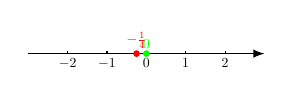
\begin{tikzpicture}[global scale = 0.5]
		\draw [black,  -latex] (-3,-2) -- (3,-2); 
		\foreach \x in {-2, ..., 2}
			\draw (\x cm,-2cm+2pt) -- (\x cm,-2cm+0pt) node[anchor=north] {$\x$};
		% -8, -6, -5, 0.1, -1/4, 0, -4.2, -5.1, 2/3, 3/2, +1/5, 0
		\draw [red, fill=red] (-1/4, -2) circle(2pt) node [above] {$-\frac{1}{4}$}; 
		\draw [green, fill=green] (0, -2) circle(2pt) node [above] {$0$}; 
	\end{tikzpicture}    
\end{document}
